\begin{LQ}{Modèle du Protocole}

\LQDescription{
    Le MdP découle du MdC et MdE. Les 3 modèles se focalisent sur le même
    système. Le MdP est le un diagramme d'états/transitions. On décrit les
    états du sytèmes et les transistions pour passer d'un état à un autre.
}

\LQSchema{
Chaque état du système est représenté par un rectangle avec un choix de nom très précis et clair pour une bonne compréhension. Les transistions se font d’un état A à un état B et sont représentés par des fleches. Une transistions peut aussi se faire d’un état A vers un état A également. Une transistion n’est possible que si elle respecte une condition. Cette condition équivaut à une action du MdE.

}

\begin{figure}
   \centering
   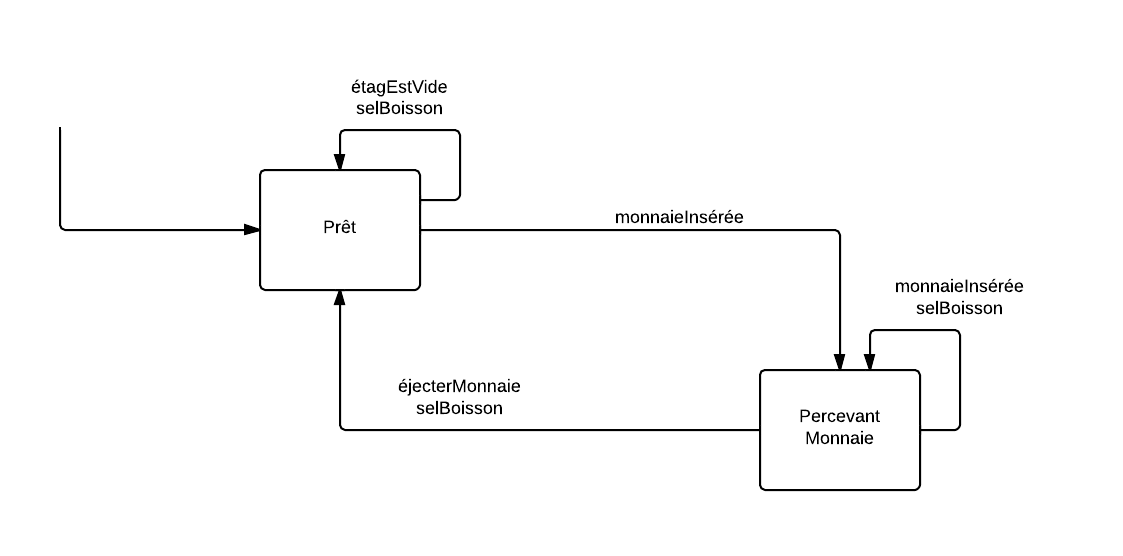
\includegraphics[width=\textwidth]{../images/MdP.png}
   \caption{Schéma du modèle du protocole}
\end{figure}

\LQModel{
    Chaque changement d'état est induit par un message. Ce qu'il veut dire que
    l'on passe d'un état à un autre que si cela est déterminer par une action.
    Le non determinisme est à proscrire ou à limiter fortement dans ce
    modèle. \\

    Chaque sous-système doit être décrit dans un modèle de protocole, et tous
    ses états doivent y être décrits. On a donc un MdP pour chaque MdC( et a
    fortiori pour chaque MdE). Chaque message provient d'une interaction et le
    système utilisé pour le MdE. \\

    Un transition qui sur son état d'origine signifie pas que le système n'a
    pas evoluer. Dans l'exemple, l'action "MonnaieInsérée"  permet
    d'incrémenter la variable "argentIntroduit" (par exemple). \\

    Le système ne doit arriver dans un état sans qu'il puisse changer d'état.
    Il doit avoir "le choix" de passer d'un état à l'autre selon les actions
    qui l'affecte. \\
}

\LQBetweenModels{
    Chaque sous-système doit être décrit dans un modèle de protocole, et tous
    ses états doivent y être décrits. \\

    Chaque message provient d'une interaction et le système utilisé pour le
    MdE. \\

    Les sous-systemes d'un MdP sont les même que ceux des MdC ou MdE.
}

\end{LQ}
